\section{Results}

\subsection{Calculation of the Monthly mean of Chlorophyll-a Concentration in the East Sea (Sea of Japan)}

The monthly-mean chlorophyll-a concentration of LAC from 2003 to 2006 is shown in Figure \ref{fig:monLAC01}. - Figure \ref{fig:monLAC03}. The monthly-mean chlorophyll-a concentration of GAC from 2003 to 2006 is shown in Figure \ref{fig:monGAC01} - Figure \ref{fig:monGAC03}. In these figures, the grey area is land of western part of Korean and southeastern part of Japan. Red area refers to relatively higher concentration compared to the blue area as it is shown at the color bar. Spring (March, April, May) and fall (October, November) show high concentration. The black area is part with no data due to cloud coverage or satellite failures. 

start 박기현
The result of monthly-mean chlorophyll-a concentration using th  LAC from 2003 to 2006 is shown in Figure \ref{fig:monLAC01}. - Figure \ref{fig:monLAC03}. The monthly-mean chlorophyll-a concentration of GAC from 2003 to 2006 is shown in Figure \ref{fig:monGAC01} - Figure \ref{fig:monGAC03}. In these figures, the grey area is land of western part of Korean and southeastern part of Japan. Red area refers to relatively higher concentration compared to the blue area as it is shown at the color bar. Spring (March, April, May) and fall (October, November) show high concentration. The black area is part with no data due to cloud coverage or satellite failures. 
end 박기현


The annual variability of chlorophyll-a concentration in the East Sea (Sea of Japan) from 2003 - 2006 is shown in Figure 1 and Figure 2. Both the LAC data and the GAC data have similar tendency, showing peaks on spring (April) and fall (November). The maximum/minimum value of LAC and GAC data was each 1.61 $\rm mg/m^3$ / 0.28 $\rm mg/m^3$, and 1.72 $\rm mg/m^3$ / 0.32 $\rm mg/m^3$. The difference between the two data was not ignorable. This infers that the effect of spatial resolution on the data has to be considered.
It is shown in Figure \ref{fig:annualmon} that the annual variability of monthly-mean chlorophyll-a concentration in the East Sea (Sea of Japan) from 2003 to 2006, (a) LAC (b) GAC.



\begin{figure}[h]
	\centering
	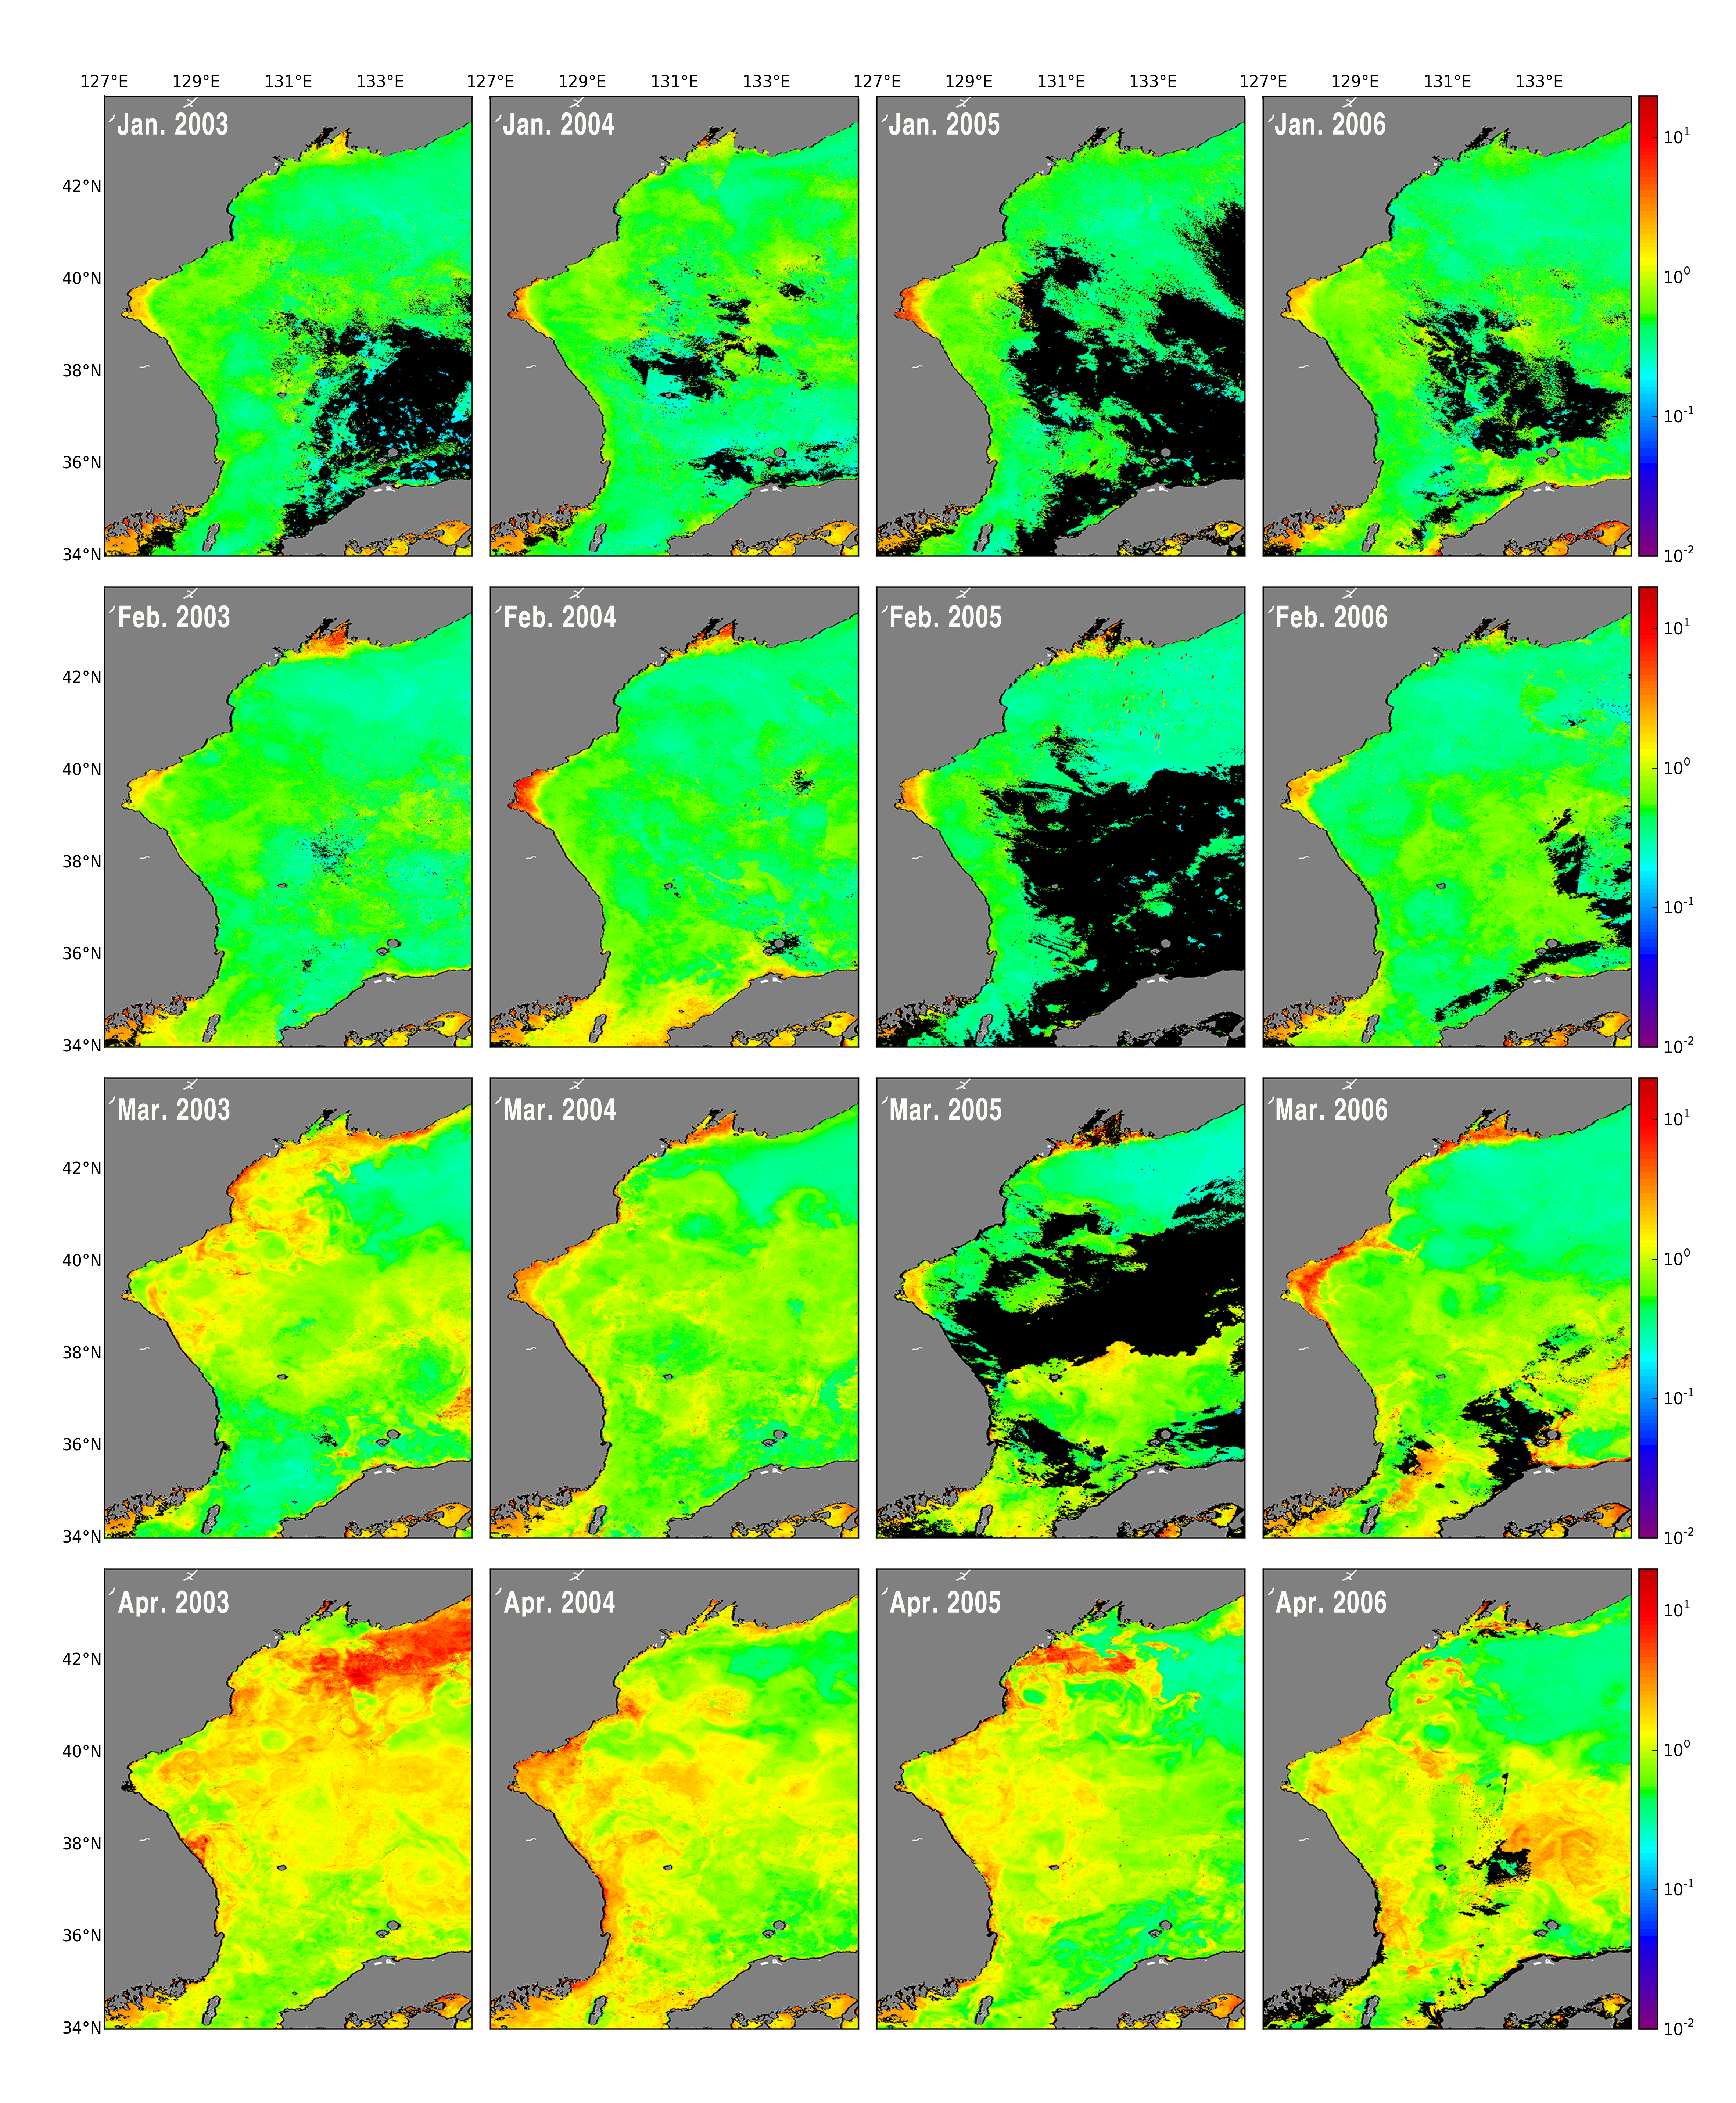
\includegraphics[width=1.0\textwidth]{monLAC01}\\
	\scriptsize\caption{The monthly-mean chlorophyll-a distribution in the East Sea (Sea of Japan), LAC. From 2003 to 2006, January to April. The unit of the color bar is $\rm mg/m^3$.}
	\label{fig:monLAC01}
\end{figure}


\begin{figure}[h]
	\centering
	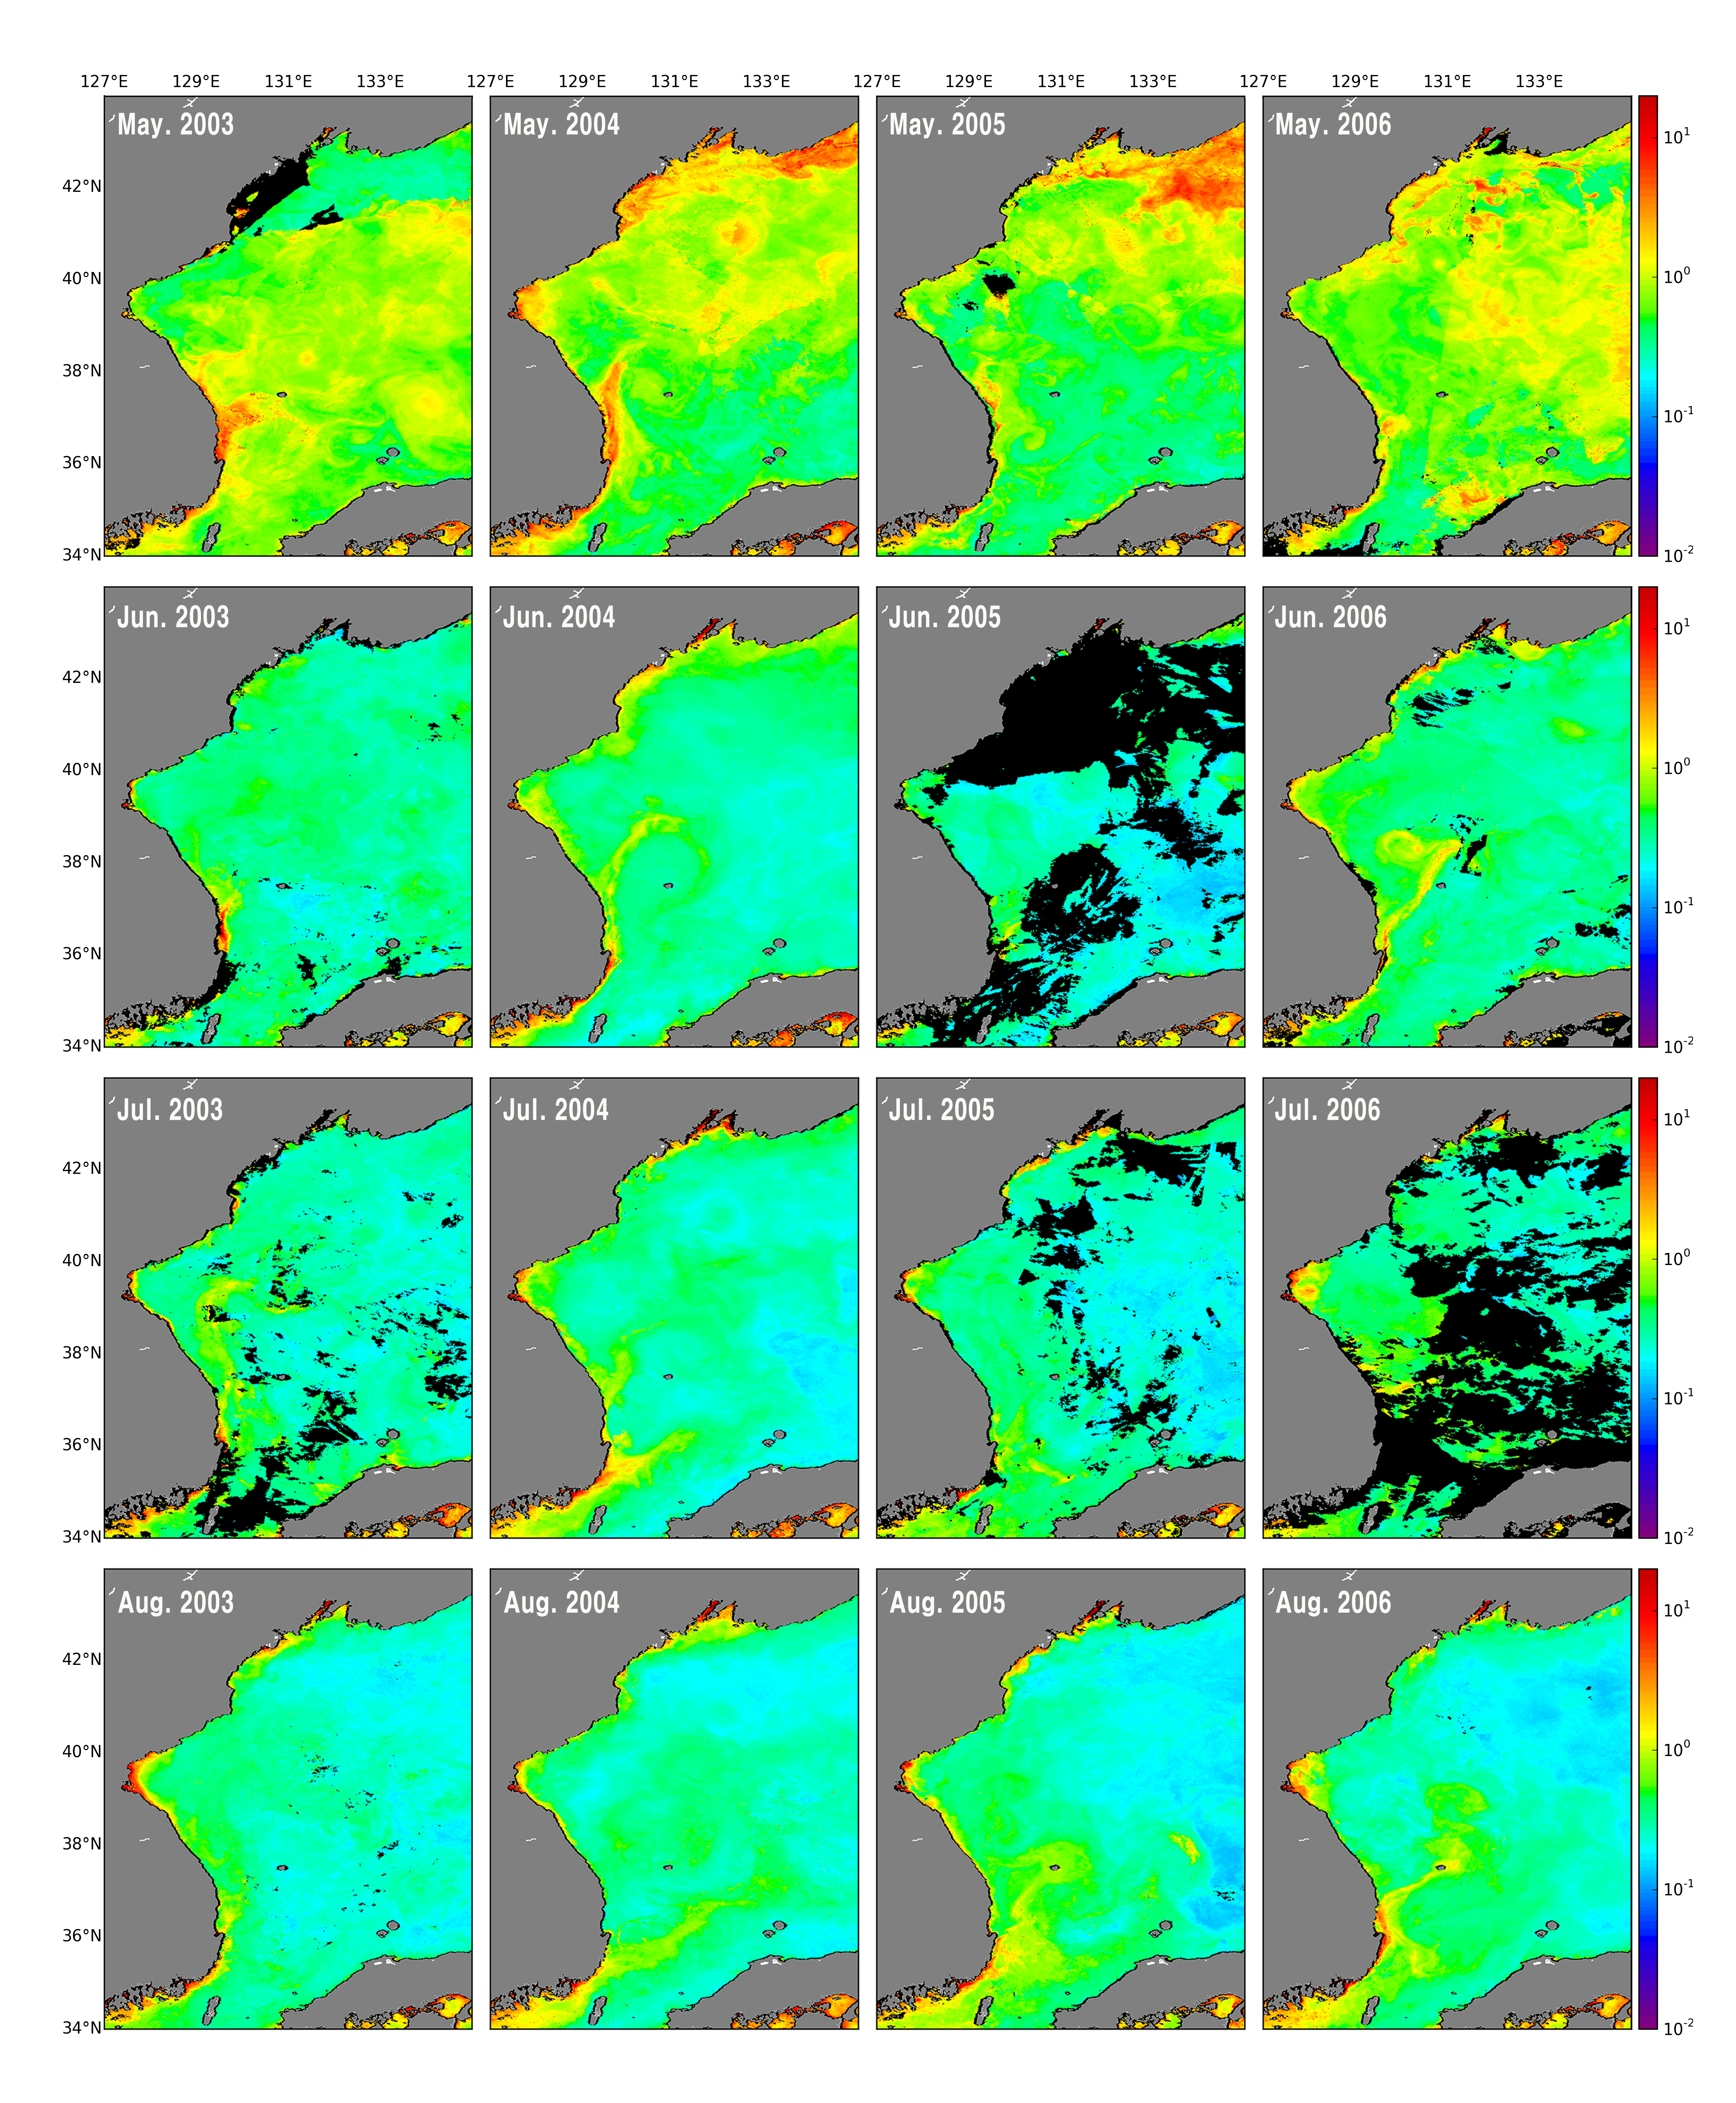
\includegraphics[width=1.00\textwidth]{../images/monLAC02}\\
	\scriptsize\caption{The monthly-mean chlorophyll-a distribution in the East Sea (Sea of Japan), LAC. From 2003 to 2006, May to August. The unit of the color bar is $\rm mg/m^3$.}
	\label{fig:monLAC02}
\end{figure}

\begin{figure}[h]
	\centering
	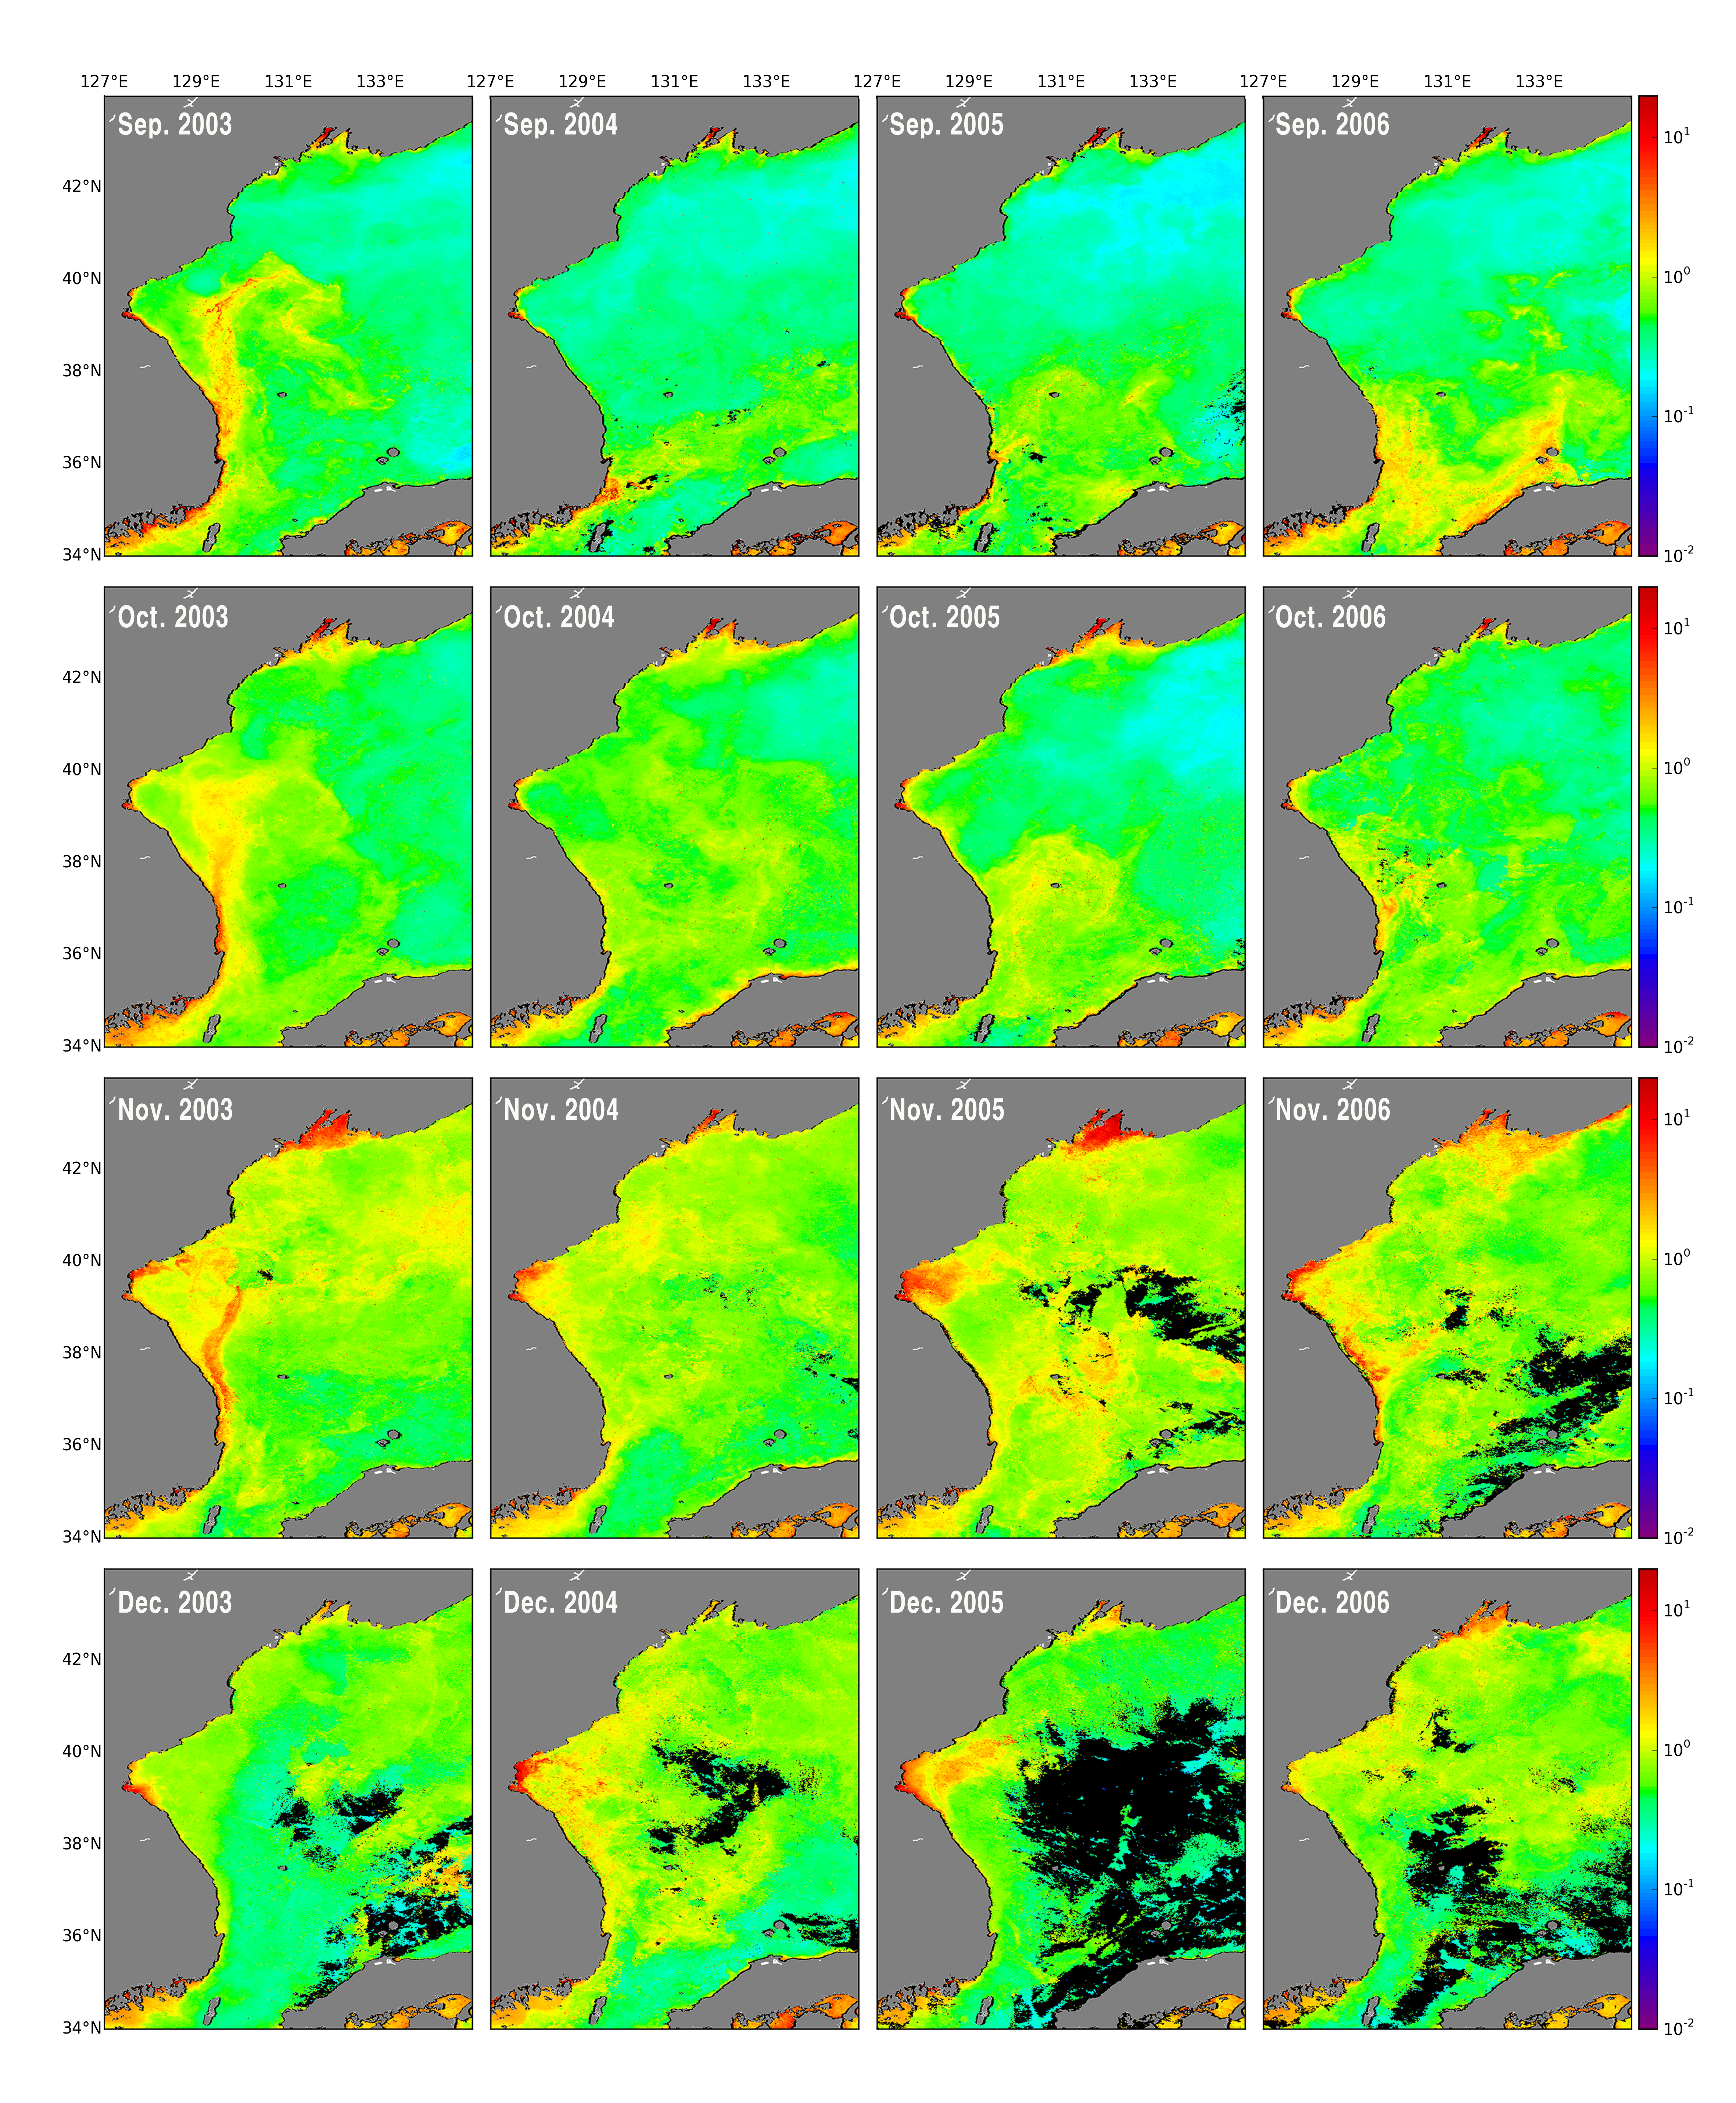
\includegraphics[width=1.00\textwidth]{../images/monLAC03}\\
	\scriptsize\caption{The monthly-mean chlorophyll-a distribution in the East Sea (Sea of Japan), LAC. From 2003 to 2006, September to December. The unit of the color bar is $\rm mg/m^3$.}
	\label{fig:monLAC03}
\end{figure}


\begin{figure}[h]
	\centering
	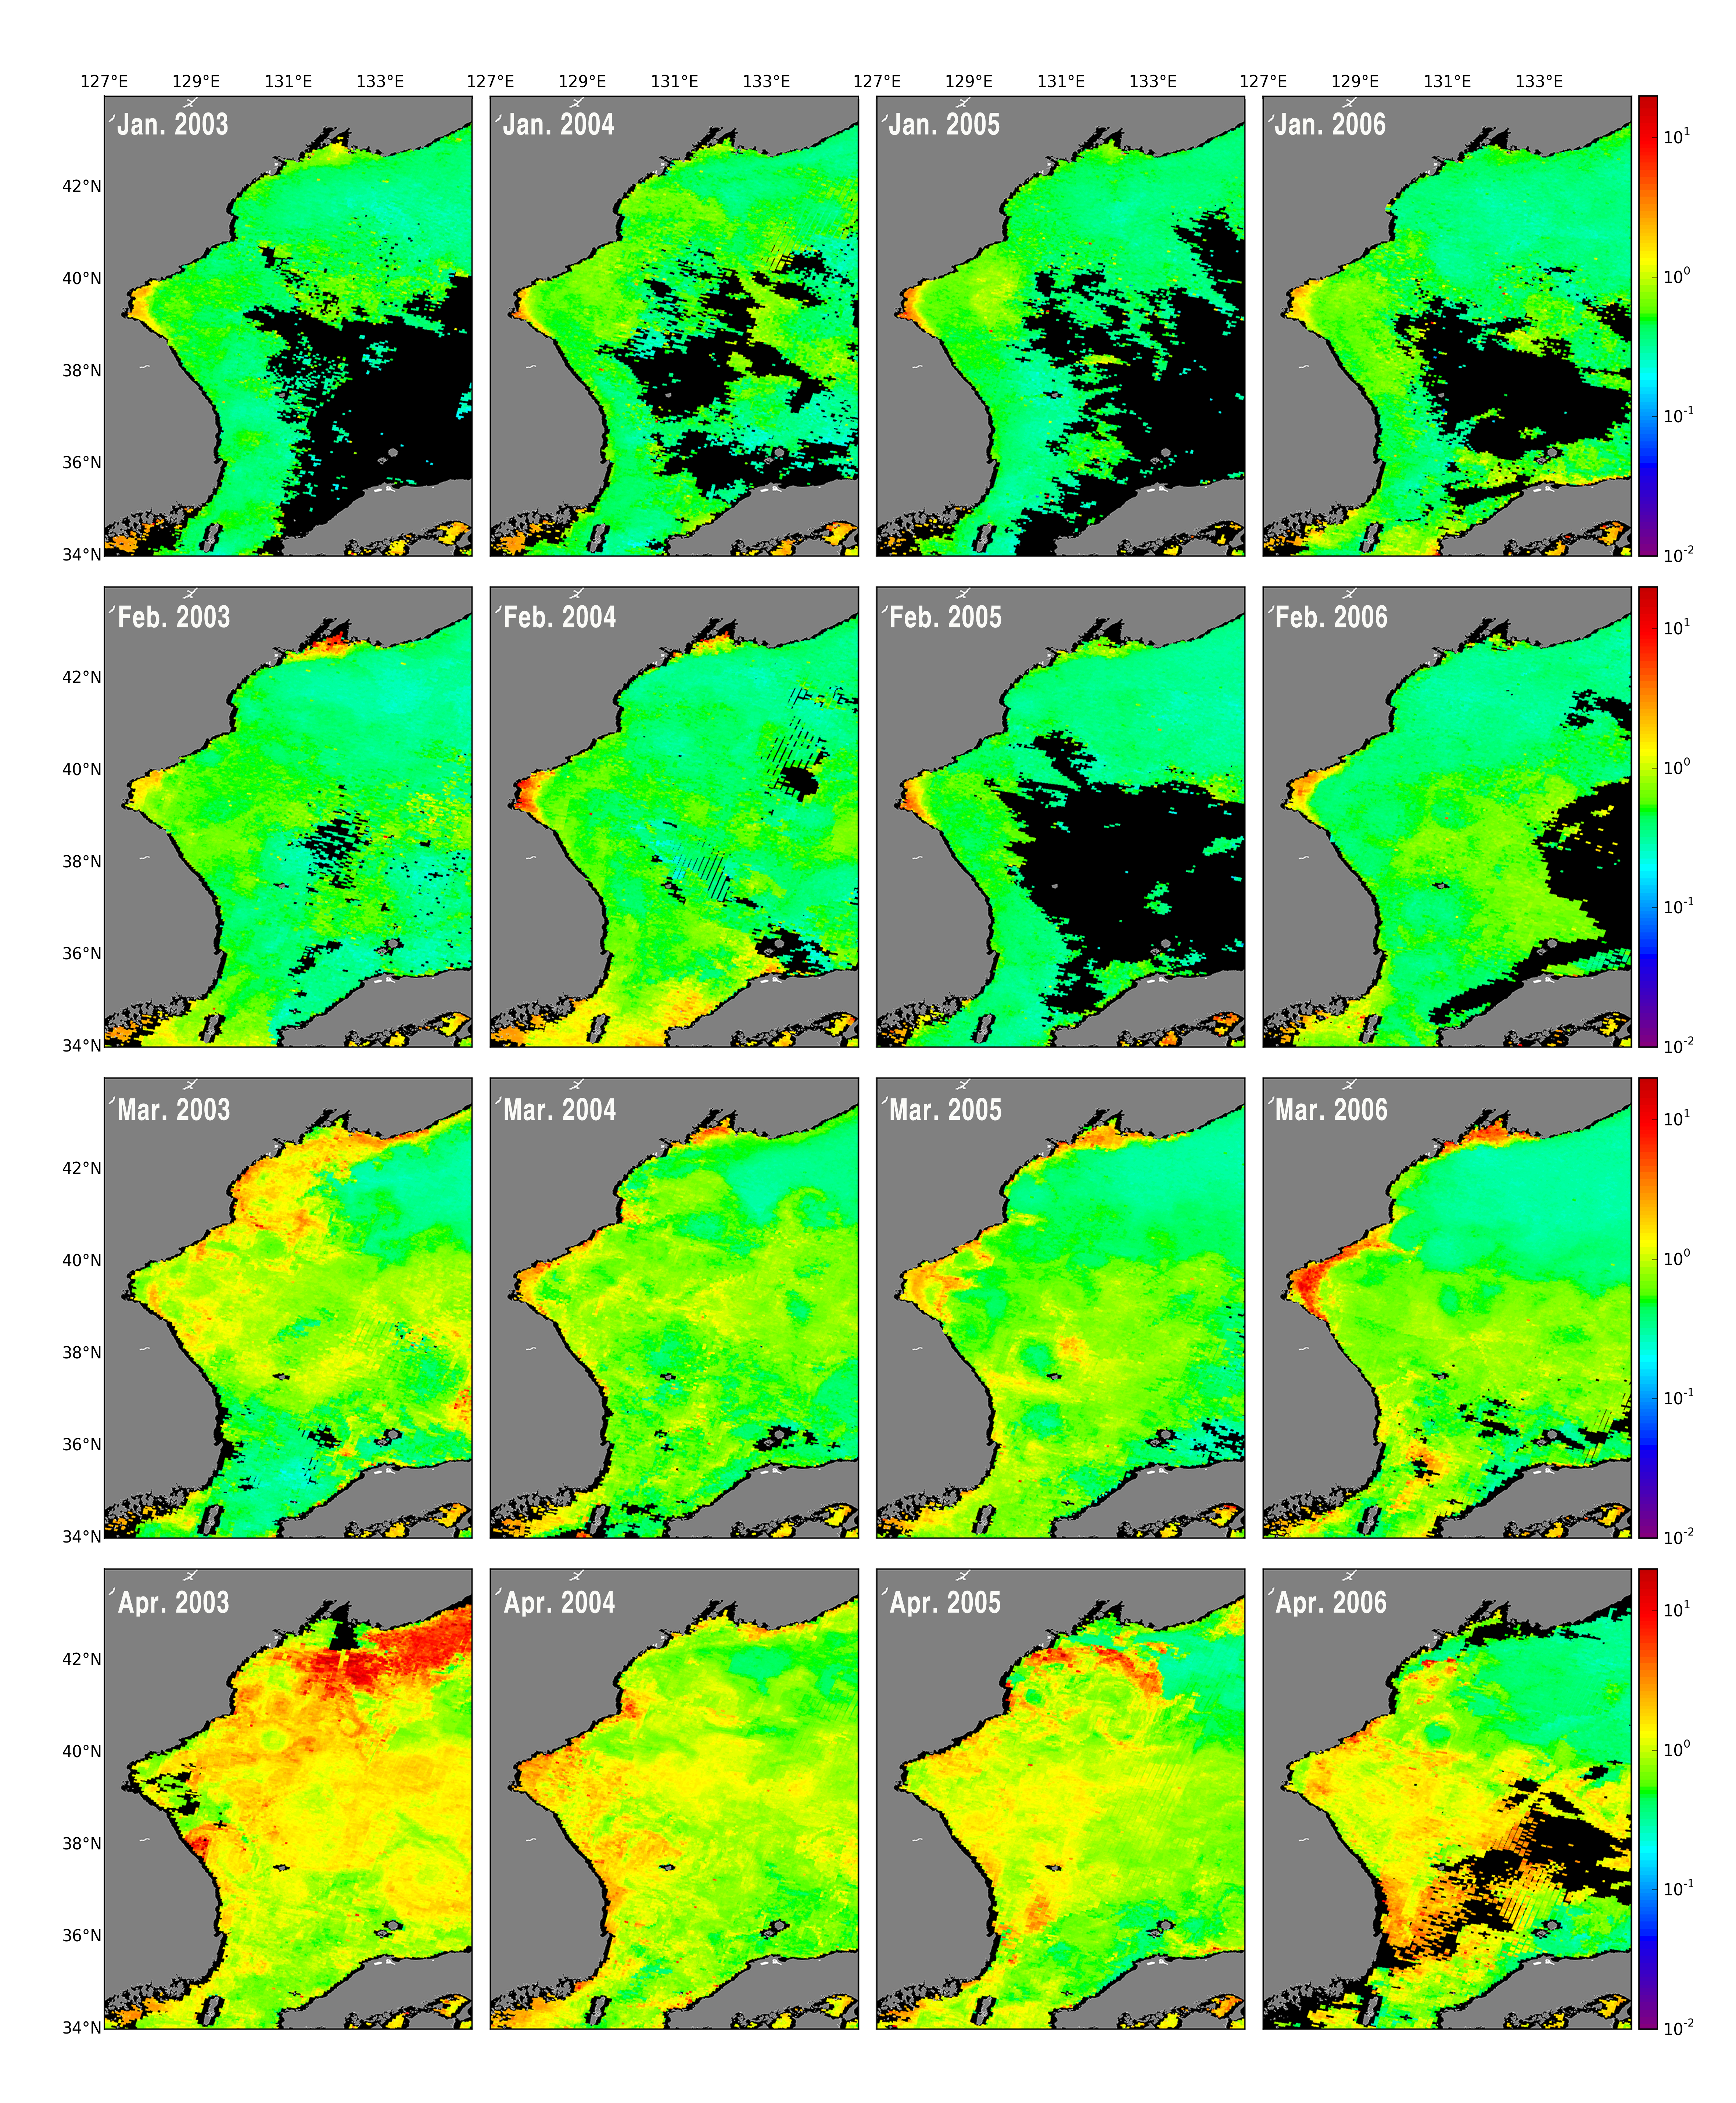
\includegraphics[width=1.0\textwidth]{../images/monGAC01}\\
	\scriptsize\caption{The monthly-mean chlorophyll-a distribution in the East Sea (Sea of Japan), LAC. From 2003 to 2006, January to April. The unit of the color bar is $\rm mg/m^3$.}
	\label{fig:monGAC01}
\end{figure}


\begin{figure}[h]
	\centering
	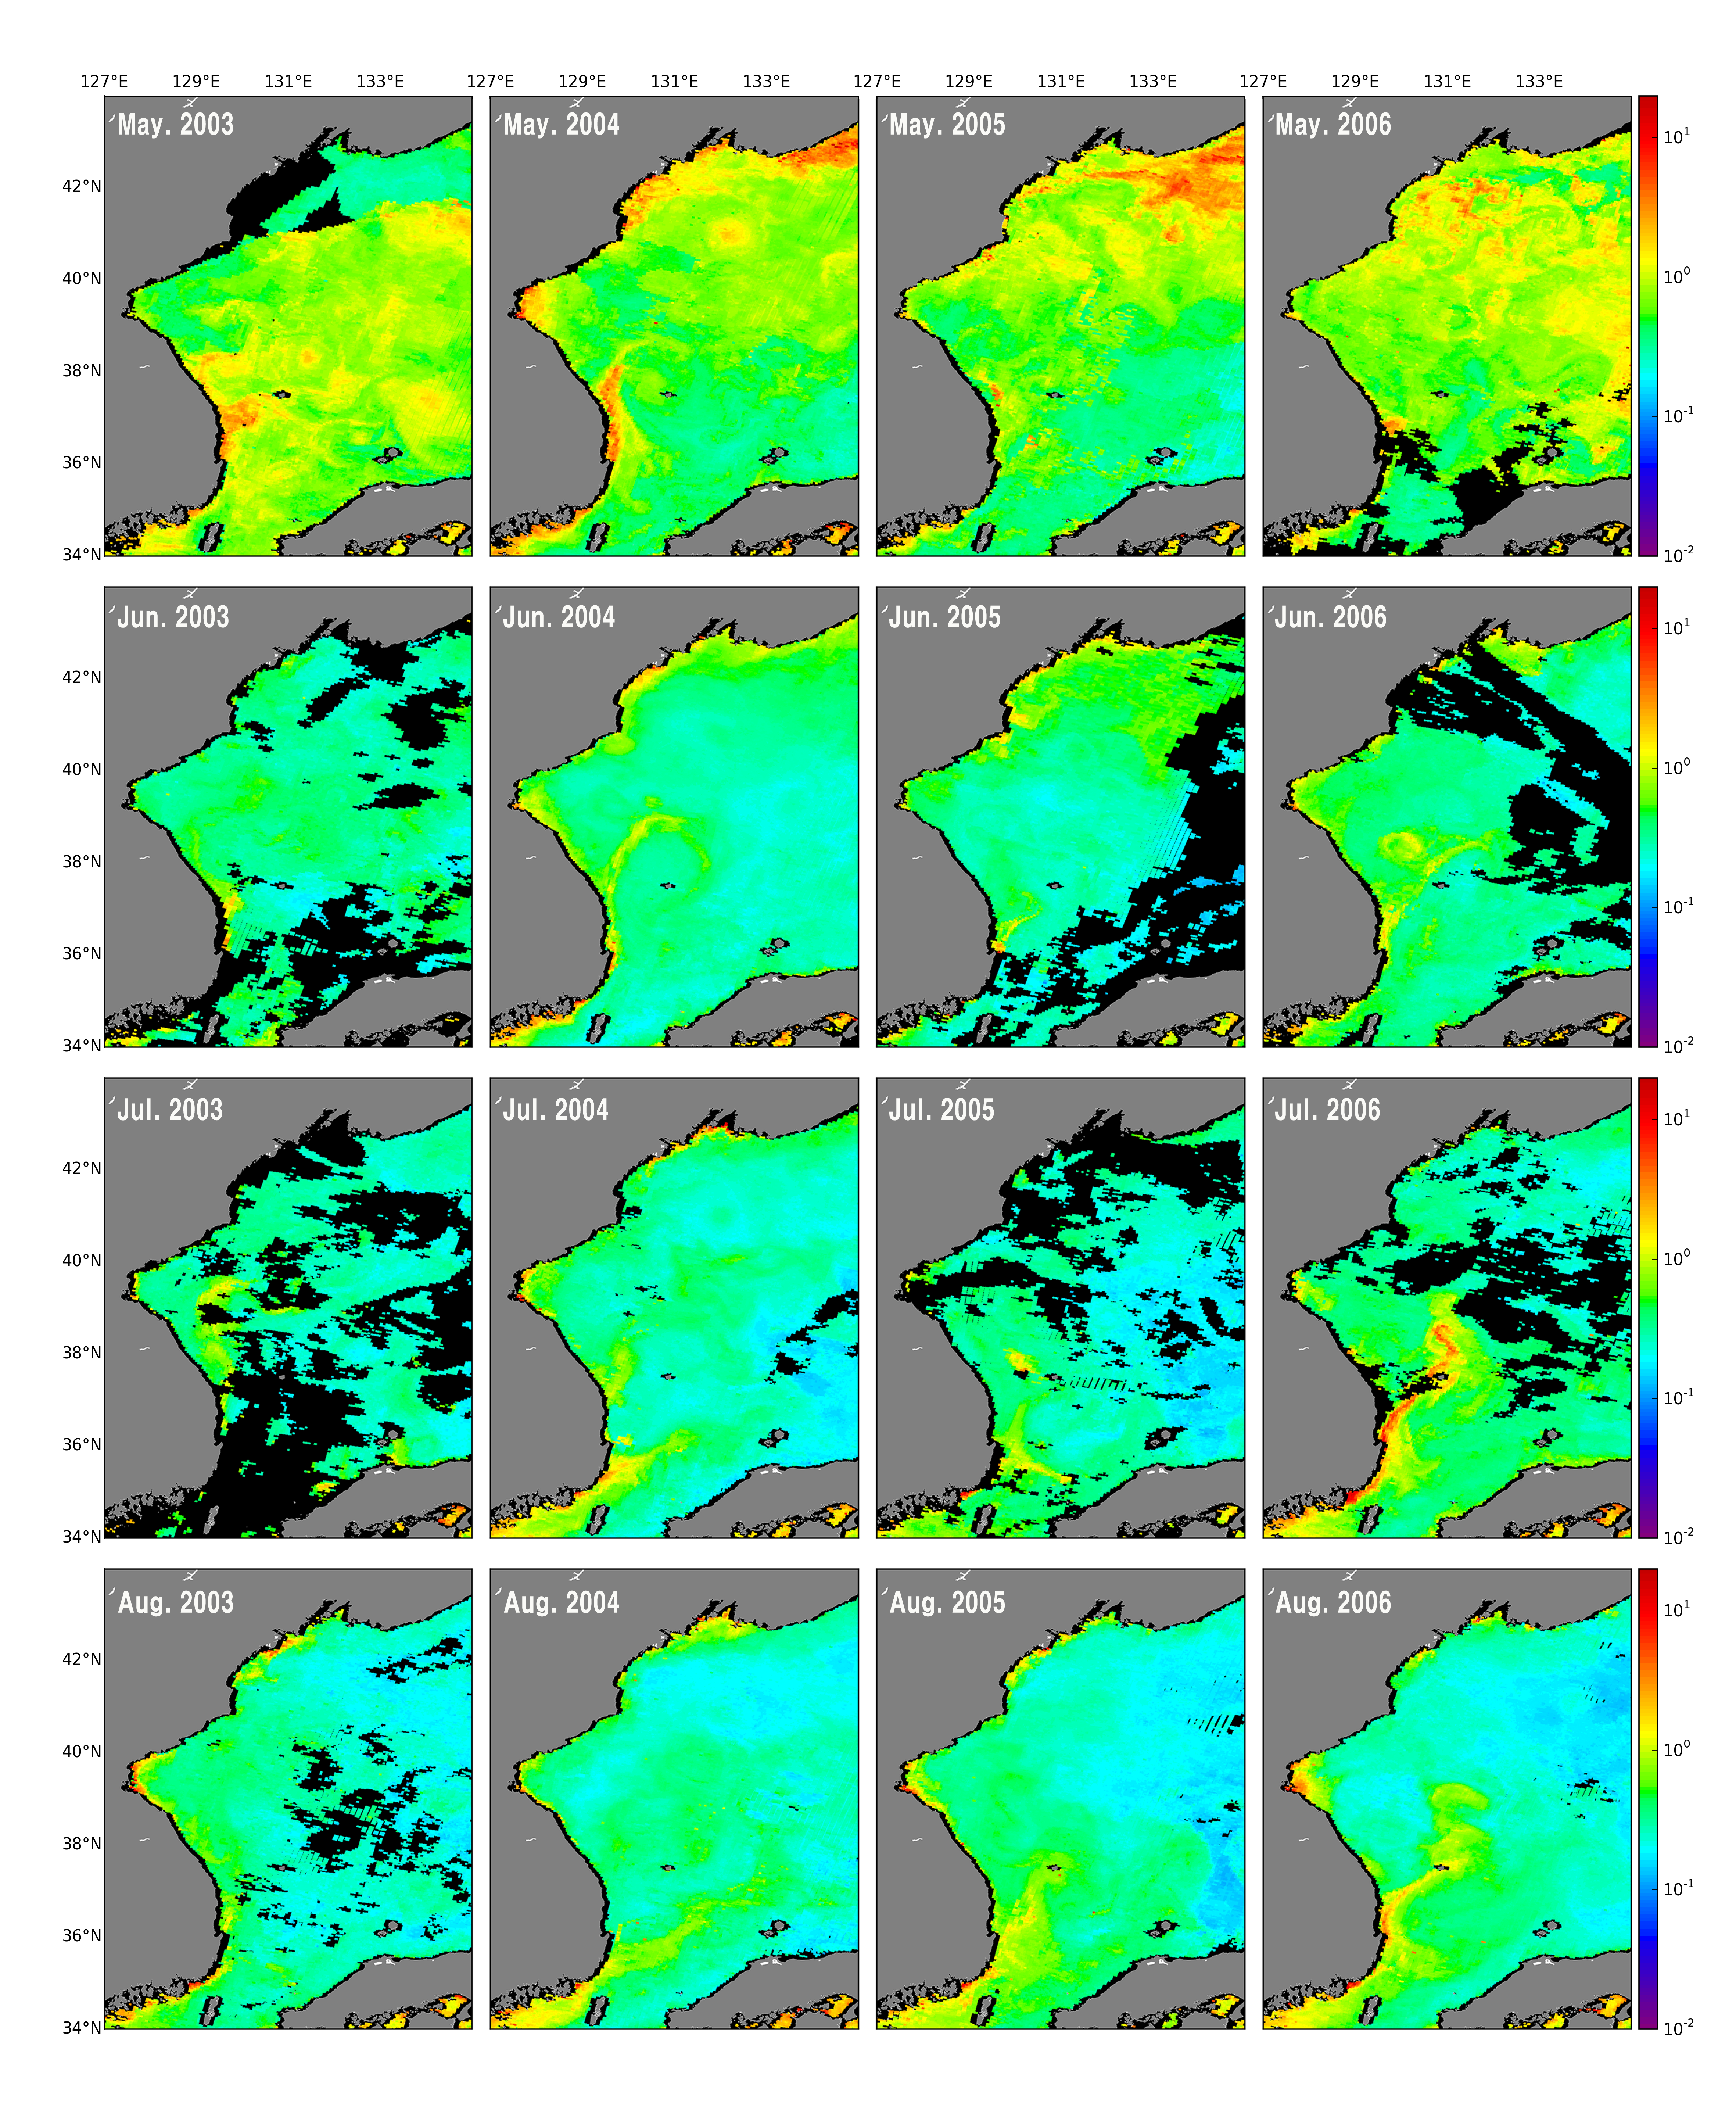
\includegraphics[width=1.00\textwidth]{../images/monGAC02}\\
	\scriptsize\caption{The monthly-mean chlorophyll-a distribution in the East Sea (Sea of Japan), LAC. From 2003 to 2006, May to August. The unit of the color bar is $\rm mg/m^3$.}
	\label{fig:monGAC02}
\end{figure}


\begin{figure}[h]
	\centering
	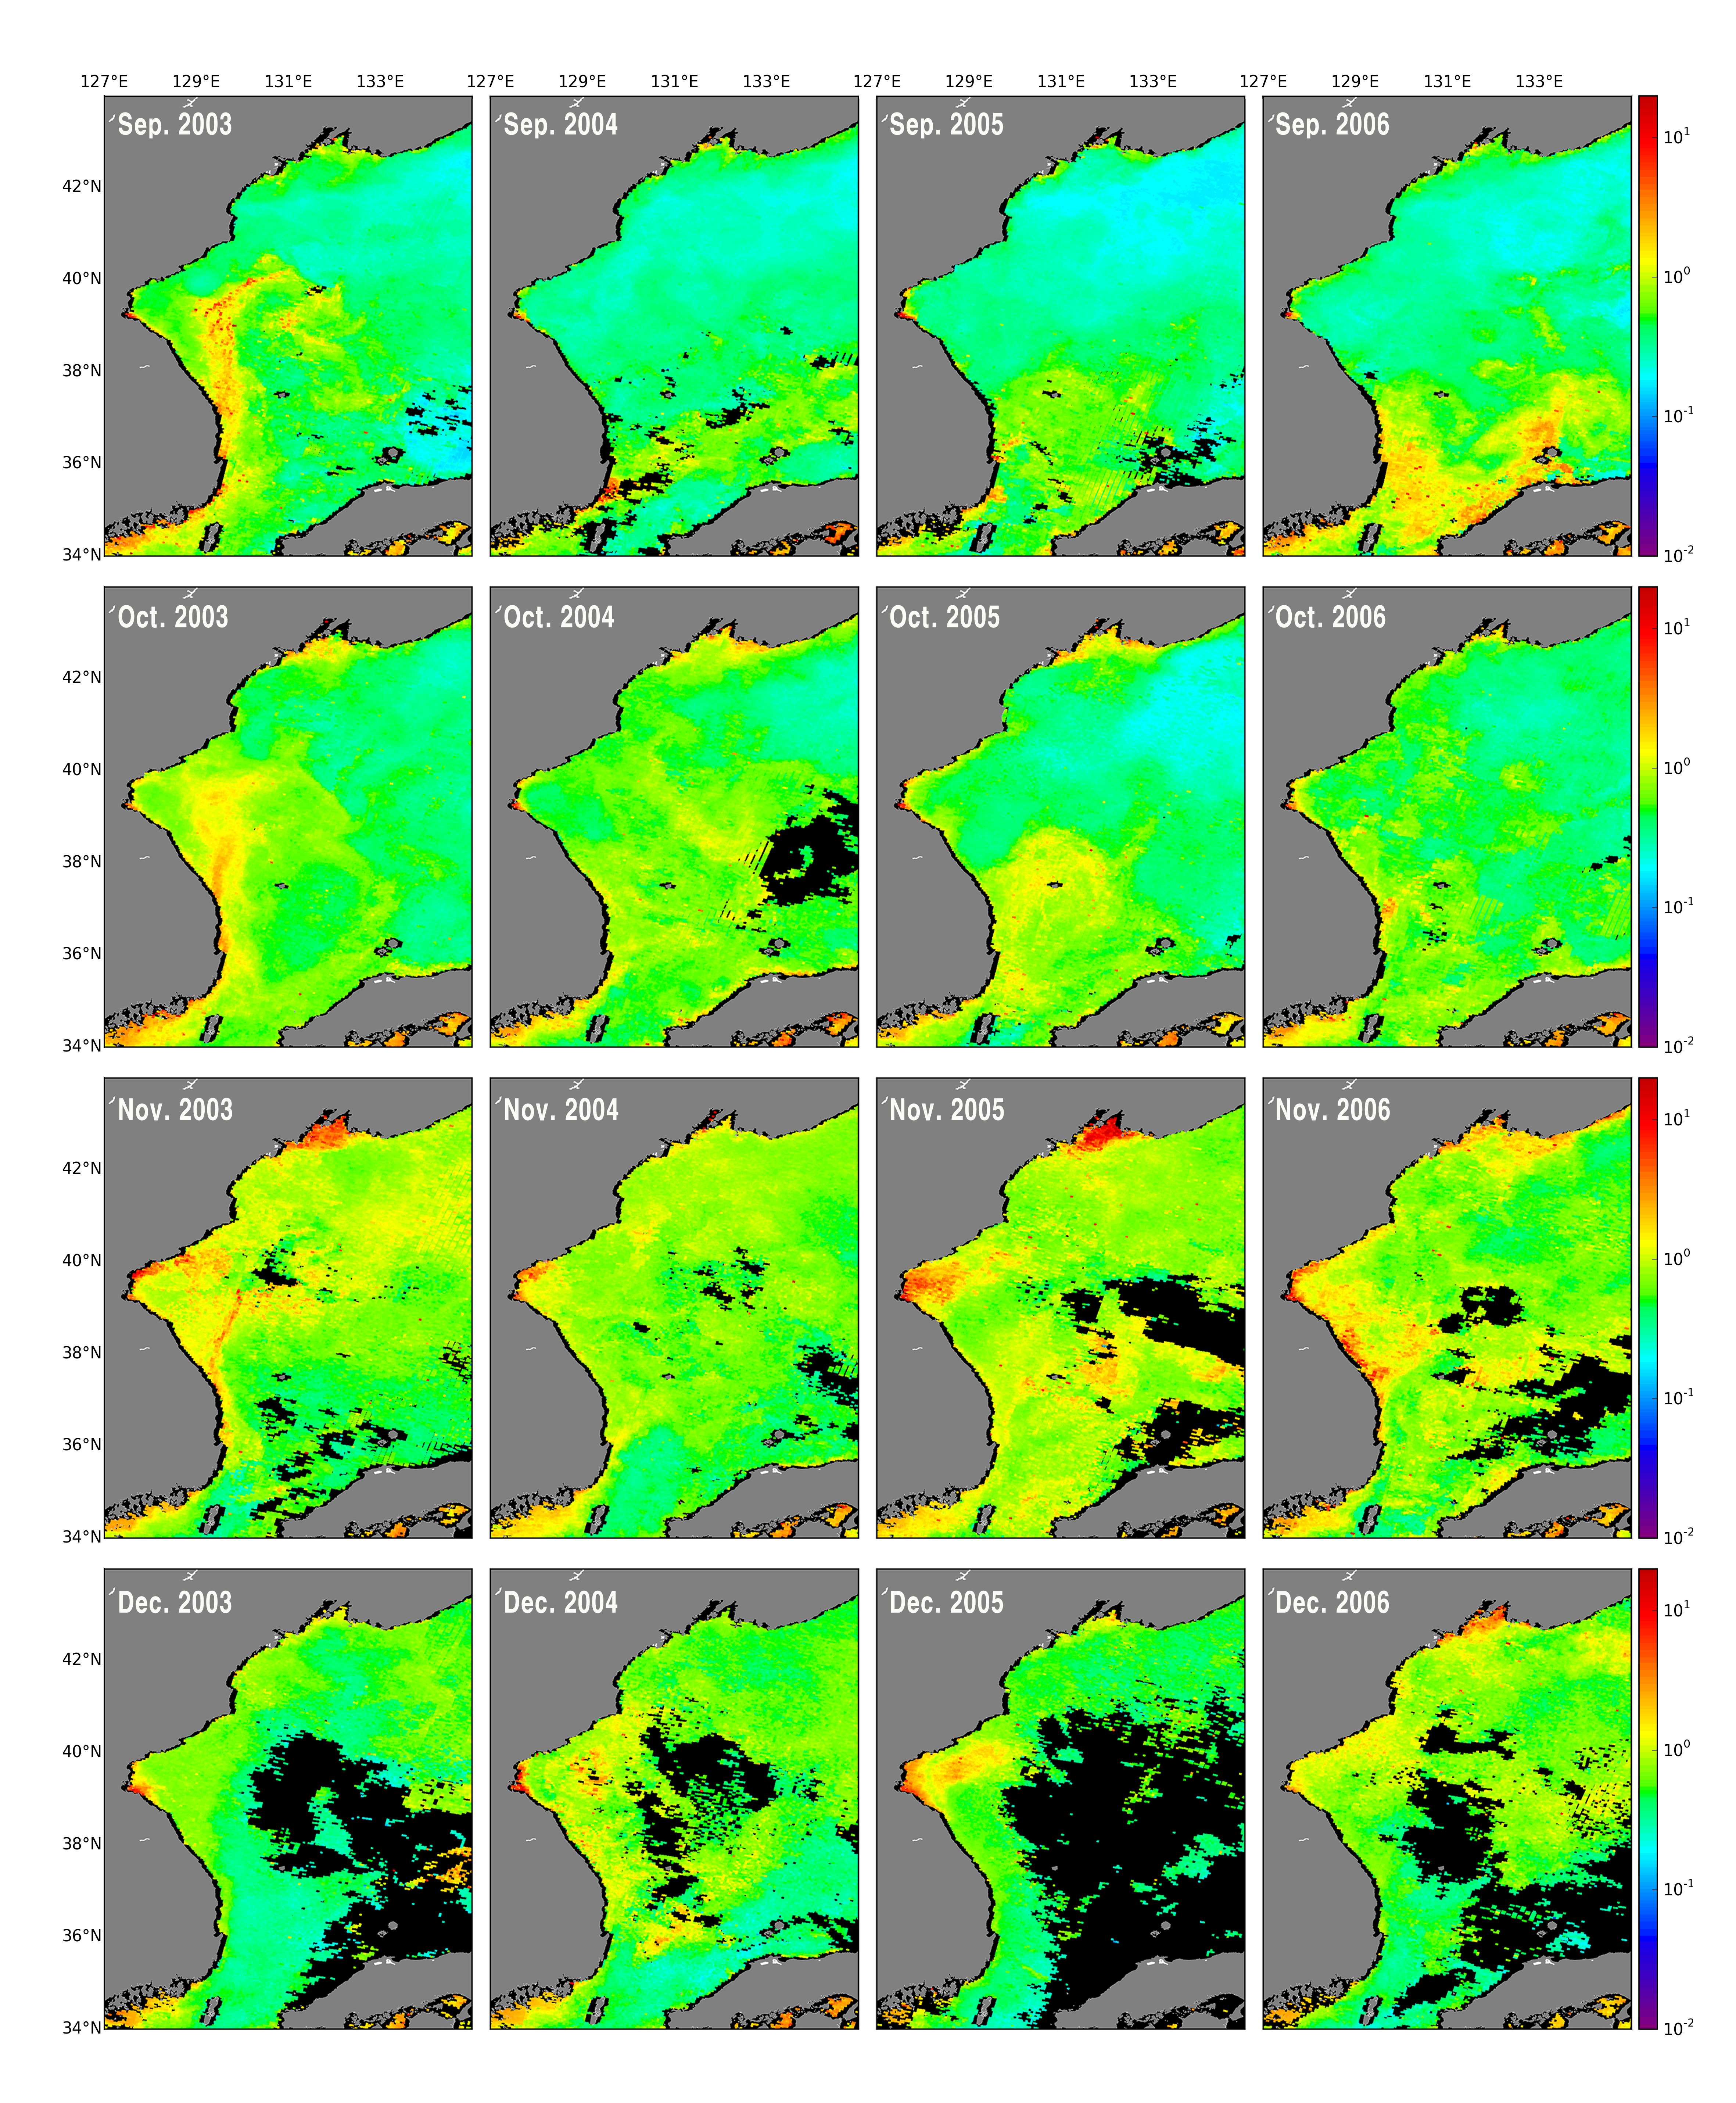
\includegraphics[width=1.00\textwidth]{../images/monGAC03}\\
	\scriptsize\caption{The monthly-mean chlorophyll-a distribution in the East Sea (Sea of Japan), LAC. From 2003 to 2006, September to December. The unit of the color bar is $\rm mg/m^3$.}
	\label{fig:monGAC03}
\end{figure}


